\chapter{数値的に常微分方程式を解く}
\label{numerical-ordinary}
第\ref{first}章で触れたように、世の中にある大半の微分方程式は解析的に解くことができません。そこで登場するのが数値解析です。計算機の力で微分方程式を数値的に解きます。具体的に関数$y(x)$を求めるのであれば、離散的な(飛び飛びの)値$x_i$に対して、各$y_i$を精度良く求めます。この$y_i$を精度良く求めるために、様々な手法が考案されました。それらを紹介します。

本書では数値解析の手法を紹介することに重点を置きます。よって、数値解析にまつわる丸め誤差や桁落ちなどについては触れません。なお、具体的なアルゴリズムの紹介には疑似コードを使います。






\section{オイラー法}
\label{euler-numerical}
オイラー法は最も簡単な数値解析の手法です。問題とする微分方程式を

\begin{eqnarray}
    \frac{\dd y}{\dd x}=f(x,y)
    \label{eq:differential-1}
\end{eqnarray}

\noindent
とします。また、初期条件を

\begin{eqnarray}
    y(x_0)=Y_0
    \label{eq:terms-1}
\end{eqnarray}

\noindent
とします。

$h$を十分小さい定数として、$y(x+h)$をテイラー展開します。

\begin{eqnarray}
    y(x+h)=y(x)+h\frac{\dd}{\dd x}y(x)+\frac{h^2}{2!}\frac{\dd^2}{\dd x^2}y(x)+\cdots
    \label{eq:taylor}
\end{eqnarray}

ここで、$h$は十分小さいので$h$の次数が2以上の項を無視します。すると、式\ref{eq:differential-1}より$\dd y(x)/\dd x$を$f(x,y)$に置換して、

\begin{eqnarray}
    y(x+h)=y(x)+hf(x,y(x))+O(h^2)
\end{eqnarray}

\noindent
となります\footnote{$O(h^2)の項は、$$O$記法(OrderのO)と言い、カッコの中身程度の量を表します。今回は$h^2$以降の項を無視したので$h^2$程度の量がこれに追加されます、という意味です。なお、この$O(h^2)$は微小量として無視する量ですので、後に誤差の話としてもう一度現れます。}。この式は何を意味するでしょうか。右辺は$y(x)$と$x$、および与えられた関数$f$で構成された式、左辺は$y(x+h)$です。そうです。第\ref{first}章で少しお話しした、「今($y(x)$)の状態から少し先の未来($y(x+h)$)を知る」方程式です。図\ref{fig:4-euler}を参照してください。

\begin{figure}[ht!]
  \centering
  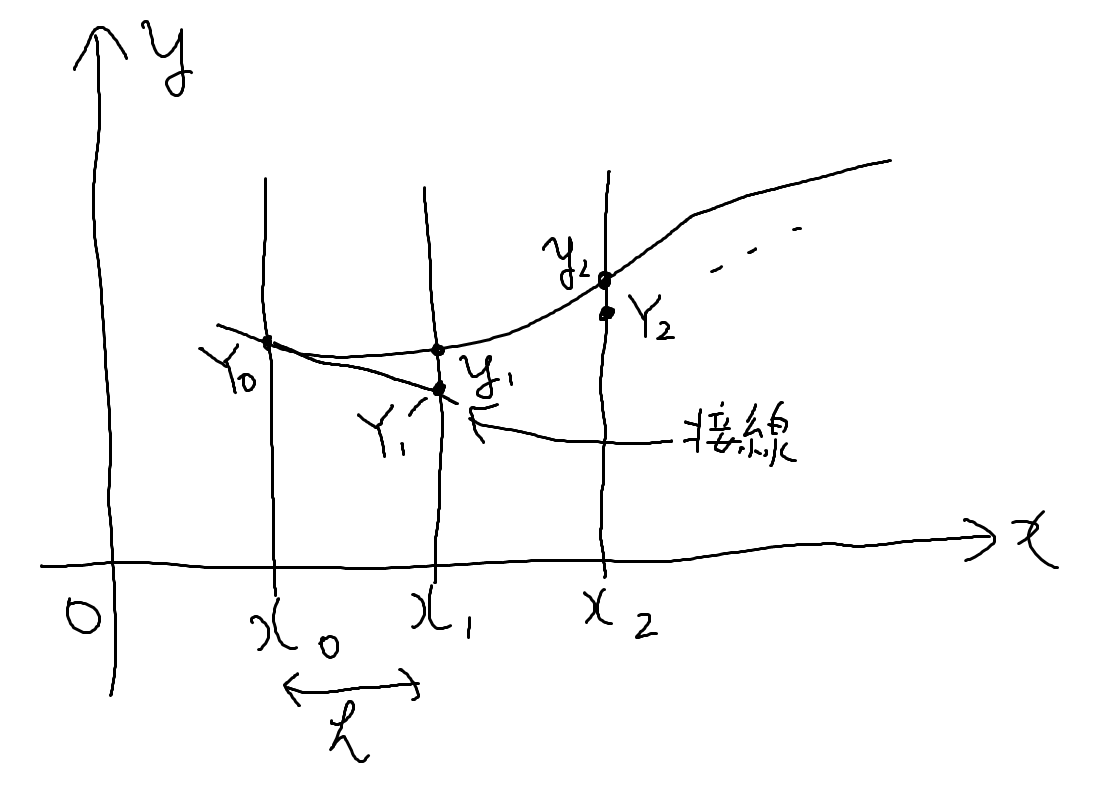
\includegraphics[width=7cm]{img/4-euler.png}
  \caption{オイラー法のイメージ}
  \label{fig:4-euler}
\end{figure}

図\ref{fig:4-euler}のように、$h$ごとに取られた各点$x_i$に対して、それぞれに対応する正しい$y$の値$y_i$、および計算機で計算した近似値$Y_i$を考えます。このとき、$h$を「刻み幅」と言います。刻み幅は一定である必要はありませんが、ここでは一定としておきます。

この考え方を使うと、$Y_{i+1}$は漸化式のように、

\begin{eqnarray}
    Y_{i+1}=Y_i+hf(x_i,Y_i)
\end{eqnarray}

\noindent
と書けます。この式を使って初期条件$x_0$で$Y_0$から順番に$x$を進めていくことで、関数$y$の近似を求めることができます。

擬似コードを以下に示します。

\begin{algorithm}
\caption{オイラー法}
\begin{algorithmic}
\REQUIRE $x_0,Y_0,h,N$
\ENSURE $Y_N$
\FOR{$i=0$ \TO $N-1$}
    \STATE $x_i\Leftarrow x_{i-1}+h$
    \STATE $Y_{i+1}\Leftarrow Y_i+hf(x_i,Y_i)$
\ENDFOR
\RETURN $Y_N$
\end{algorithmic}
\end{algorithm}

$h$の2乗以上の項を無視したので、局所誤差\footnote{一回の計算につき生じうる誤差のことです}は$O(h^2)$です。

また、誤差の蓄積を考えれば、最終的に得られる計算結果に含まれる誤差\footnote{計算を繰り返し、最終的に生じうる誤差のことです}は

\begin{eqnarray}
    O(h^2)\times \frac{x_N-x_0}{h}=O(h)
\end{eqnarray}

となり、$O(h)$の誤差が含まれていると言えます。







\section{改良オイラー法(中点法)}
\label{adv-euler}
オイラー法は計算が軽い反面、言ってしまえば精度がいまいちでした。そこで、簡単に精度を上げる方法として図\ref{fig:4-adv-euler}の方法を考えます。

\begin{figure}[ht!]
  \centering
  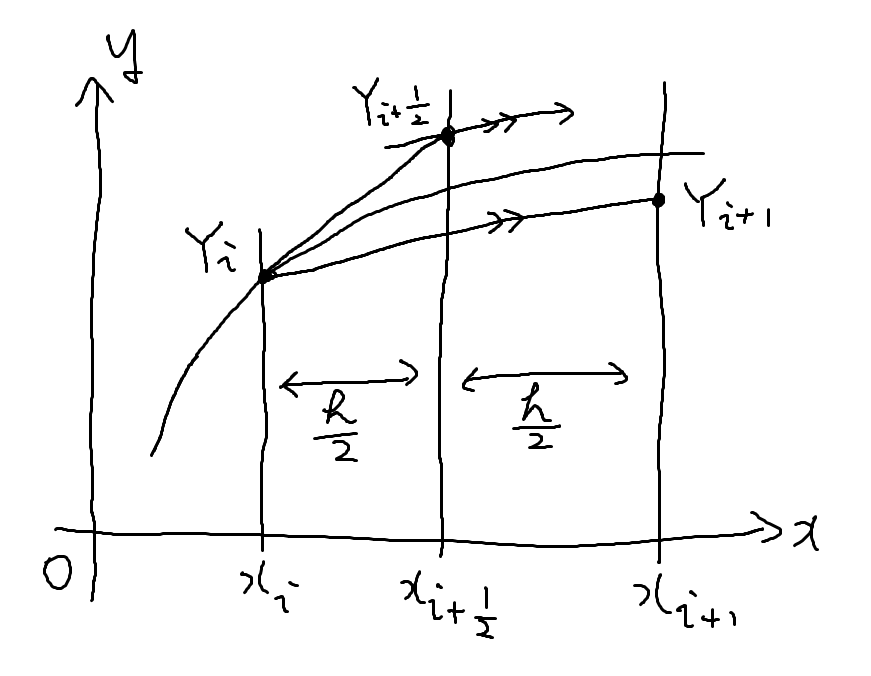
\includegraphics[width=10cm]{img/4-adv-euler.png}
  \caption{改良オイラー法のイメージ}
  \label{fig:4-adv-euler}
\end{figure}

これは、

\begin{enumerate}
    \item 通常のオイラー法を使って$Y_{i+1/2}$を求める
    \item 微分方程式から$Y_{i+1/2}$での勾配$k$を求める
    \item $Y_{i+1}=Y_i+hk$として$Y_{i+1}$を定める
\end{enumerate}

という手順を踏んでいます。改良オイラー法は勾配として点$Y_{i+1/2}$での傾きを使うことに特徴があります。これを擬似コードにすると以下になります。解く微分方程式はオイラー法と同じ式\ref{eq:differential-1}とします。

\begin{algorithm}
\caption{改良オイラー法}
\begin{algorithmic}
\REQUIRE $x_0,Y_0,h,N$
\ENSURE $Y_N$
\FOR{$i=0$ \TO $N-1$}
    \STATE $x_{i+1/2}\Leftarrow x_i+\frac{h}{2}$
    \STATE $Y_{i+1/2}\Leftarrow Y_i+\frac{h}{2}f(x_i,Y_i)$
    \STATE $Y_{i+1}\Leftarrow Y_i+hf(x_{i+1/2},Y_{i+1/2})$
\ENDFOR
\RETURN $Y_N$
\end{algorithmic}
\end{algorithm}

計算はオイラー法よりも多少重くなってしまいました(とは言っても定数倍です)が、精度はかなり良くなりました。実際に誤差を見積もってみましょう。改良オイラー法は、擬似コードを1つの式にすれば、

\begin{eqnarray}
    Y_{i+1}=Y_i+hf\pqty{x_{i+1/2},Y_i+\frac{h}{2}f(x_i,Y_i)}
\end{eqnarray}

\noindent
です。$f(x,y)=\dd y/\dd x$とオイラー法で出てきたテイラー展開式\ref{eq:taylor}を使って展開してみましょう。

\begin{eqnarray}
    Y_{i+1}&=&Y_i+h\pqty{\frac{\dd}{\dd x}y\pqty{x_i+\frac{h}{2}}} \\
    &=&Y_i+h\frac{\dd}{\dd x}\pqty{y(x_i)+\frac{h}{2}\frac{\dd}{\dd x}y(x_i)} \nonumber \\
    &=&Y_i+h\frac{\dd}{\dd x}y(x_i)+\frac{h^2}{2}\frac{\dd^2}{\dd x^2}y(x_i) \setcounter{equation}{9}
\end{eqnarray}

テイラー展開式\ref{eq:taylor}と比べると、2次の項まで一致しています。よって局所誤差は$O(h^3)$です。よって、最終的に生じうる誤差は

\begin{eqnarray}
    O(h^3)\times \frac{x_N-x_0}{h}=O(h^2)
\end{eqnarray}

です。オイラー法は$O(h)$でしたので、ぐんと誤差が小さくなりましたね。







\section{ルンゲ・クッタ法}
\label{runge-kutta}
ここではまず狭義のルンゲ・クッタ法を紹介し、その後に一般化されたルンゲ・クッタ法を紹介します。

オイラー法や改良オイラー法は

\begin{eqnarray}
    Y_{i+1}=Y_i+h\Phi(x_i,Y_i)
\end{eqnarray}

\noindent
という形の式をしていました。ルンゲ・クッタ法ではこの式について$\Phi$を工夫することで精度を高める試みをしています。オイラー法や改良オイラー法では勾配を1つだけ求め、それを採用していましたが、ルンゲ・クッタ法では勾配を複数求め、その重みつき平均を勾配とします。

狭義のルンゲ・クッタ法は、「4段4次のルンゲ・クッタ法」と呼ばれ、

\begin{eqnarray}
    k_1&=&f(x_i,Y_i) \\
    k_2&=&f\pqty{x_i+\frac{h}{2},Y_i+\frac{k_1}{2}} \\
    k_3&=&f\pqty{x_i+\frac{h}{2},Y_i+\frac{k_2}{2}} \\
    k_4&=&f(x_i+h,Y_i+hk_3)
\end{eqnarray}

\noindent
として勾配$k_1$から$k_4$を定義して、

\begin{eqnarray}
    Y_{i+1}=Y_i+\frac{h}{6}(k_1+2k_2+2k_3+k_4)
    \label{eq:runge-kutta}
\end{eqnarray}

\noindent
として$Y_{i+1}$を求めます。たくさん$k$が出てきましたが、これらは、

\clearpage

\begin{itemize}
    \item $k_1$は$x_i$での勾配(通常のオイラー法で使う勾配)
    \item $k_2$は$x_{i+1/2}$での勾配(改良オイラー法で使う勾配)
    \item $k_3$は$k_2$の値から推測した$Y_{i+1/2}$を使用した、$x_{i+1/2}$での勾配
    \item $k_4$は$k_3$の値から推測した$Y_{i+1}$を使用した、$x_{i+1}$での勾配
\end{itemize}

\noindent
という意味を持ちます。$k$を図にすると図\ref{fig:4-runge-kutta}となります。

\begin{figure}[ht!]
  \centering
  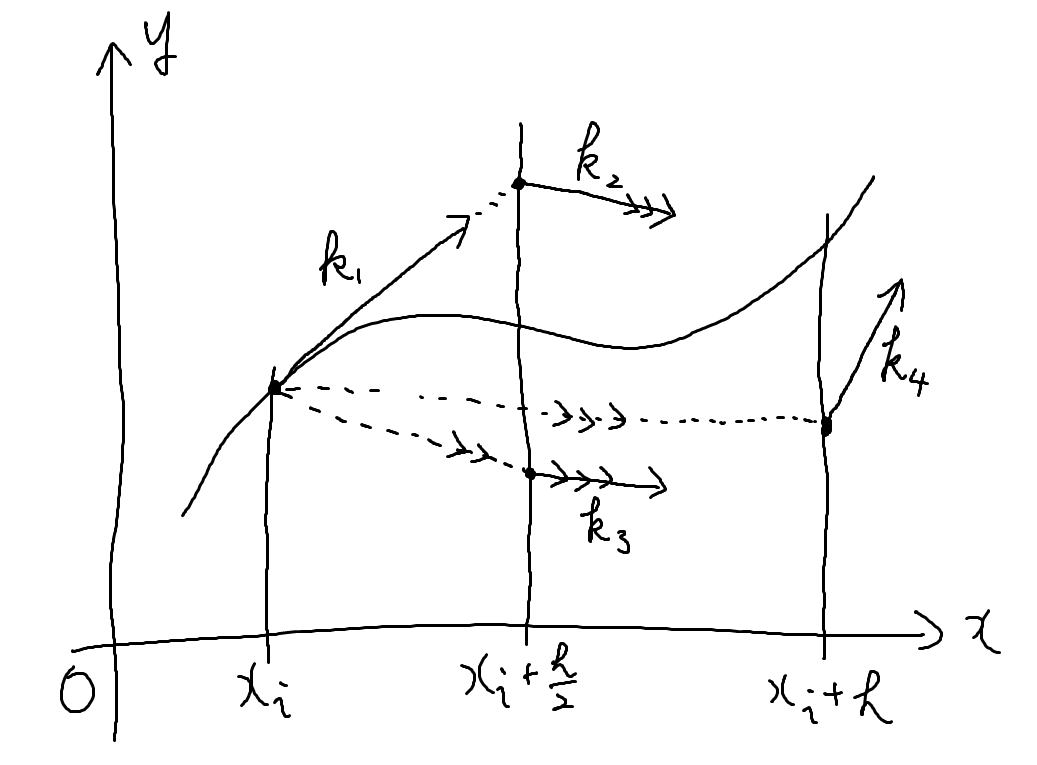
\includegraphics[width=10cm]{img/4-runge-kutta.png}
  \caption{4段4次ルンゲ・クッタ法のイメージ}
  \label{fig:4-runge-kutta}
\end{figure}

これらの$k$を重みをつけて平均し、$Y_{i+1}$を求めるときに使う勾配とします。

擬似コードにすると以下です。

\begin{algorithm}
\caption{4段4次ルンゲ・クッタ法}
\begin{algorithmic}
\REQUIRE $x_0,Y_0,h,N$
\ENSURE $Y_N$
\FOR{$i=0$ \TO $N-1$}
    \STATE $x_i\Leftarrow x_{i-1}+h$
    \STATE $k_1\Leftarrow f(x_i,Y_i)$
    \STATE $k_2\Leftarrow f\pqty{x_i+\frac{h}{2},Y_i+\frac{k_1}{2}}$
    \STATE $k_3\Leftarrow f\pqty{x_i+\frac{h}{2},Y_i+\frac{k_2}{2}}$
    \STATE $k_4\Leftarrow (x_i+h,Y_i+hk_3)$
    \STATE $Y_{i+1}\Leftarrow Y_i+\frac{h}{6}(k_1+2k_2+2k_3+k_4)$
\ENDFOR
\RETURN $Y_N$
\end{algorithmic}
\end{algorithm}

4段4次のルンゲ・クッタ法の誤差を見積もってみましょう。各$k$について$\dd y/\dd x$を使った形に書き換え、最後にルンゲ・クッタ法の式\ref{eq:runge-kutta}に代入します。

まずは$k_1$についてです。

\begin{eqnarray}
    k_1&=&\frac{\dd}{\dd x}y(x_i)
\end{eqnarray}

$k_2$については、

\begin{eqnarray}
    k_2&=&\frac{\dd}{\dd x}y\pqty{x_i+\frac{h}{2}} \\
    &=&\frac{\dd}{\dd x}\pqty{y(x_i)+\frac{h}{2}\frac{\dd}{\dd x}y(x_i)} \nonumber \\
    &=&\frac{\dd}{\dd x}y(x_i)+\frac{h}{2}\frac{\dd^2}{\dd x^2}y(x_i) \setcounter{equation}{19}
\end{eqnarray}

$k_3$は、

\begin{eqnarray}
    k_3&=&\frac{\dd}{\dd x}y\pqty{x_i+\frac{h}{2}} \\
    &=&\frac{\dd}{\dd x}\pqty{y(x_i)+\frac{h}{2}\frac{\dd}{\dd x}y\pqty{x_i+\frac{h}{2}}} \ \mbox{($k_2$の傾きを使う)} \nonumber \\
    &=&\frac{\dd}{\dd x}\pqty{y(x_i)+\frac{h}{2}\pqty{\frac{\dd}{\dd x}y(x_i)+\frac{h}{2}\frac{\dd^2}{\dd x^2}y(x_i)}} \nonumber \\
    &=&\frac{\dd}{\dd x}y(x_i)+\frac{h}{2}\frac{\dd^2}{\dd x^2}y(x_i)+\frac{h^2}{4}\frac{\dd^3}{\dd x^3}y(x_i) \setcounter{equation}{21}
\end{eqnarray}

最後に$k_4$です。

\begin{eqnarray}
    k_4&=&\frac{\dd}{\dd x}y(x_i+h) \\
    &=&\frac{\dd}{\dd x}\pqty{y(x_i)+h\frac{\dd}{\dd x}y\pqty{x_i+\frac{h}{2}}}\ \mbox{($k_3$の傾きを使う)} \nonumber \\
    &=&\frac{\dd}{\dd x}\pqty{y(x_i)+h\pqty{\frac{\dd}{\dd x}y(x_i)+\frac{h}{2}\frac{\dd^2}{\dd x^2}y(x_i)+\frac{h^2}{4}\frac{\dd^3}{\dd x^3}y(x_i)}} \nonumber \\
    &=&\frac{\dd}{\dd x}y(x_i)+h\frac{\dd^2}{\dd x^2}y(x)+\frac{h^2}{2}\frac{\dd^3}{\dd x^3}y(x_i)+\frac{h^3}{4}\frac{\dd^4}{\dd x^4}y(x_i) \setcounter{equation}{23}
\end{eqnarray}

さて、では4段4次のルンゲ・クッタ法の式\ref{eq:runge-kutta}に代入しましょう。

\begin{eqnarray}
    Y_{i+1}&=&Y_i+\frac{h}{6}\frac{\dd}{\dd x}y(x_i)
    +\frac{h}{3}\pqty{\frac{\dd}{\dd x}y(x_i)+\frac{h}{2}\frac{\dd^2}{\dd x^2}y(x_i)} \nonumber \\
    &+&\frac{h}{3}\pqty{\frac{\dd}{\dd x}y(x_i)+\frac{h}{2}\frac{\dd^2}{\dd x^2}y(x_i)+\frac{h^2}{4}\frac{\dd^3}{\dd x^3}y(x_i)} \nonumber \\
    &+&\frac{h}{6}\pqty{\frac{\dd}{\dd x}y(x_i)+h\frac{\dd^2}{\dd x^2}y(x)+\frac{h^2}{2}\frac{\dd^3}{\dd x^3}y(x_i)+\frac{h^3}{4}\frac{\dd^4}{\dd x^4}y(x_i)} \setcounter{equation}{24}\\
    &=&Y_i+h\frac{\dd}{\dd x}y(x_i)+\frac{h^2}{2}\frac{\dd^2}{\dd x^2}y(x_i)+\frac{h^3}{6}\frac{\dd^3}{\dd x^3}y(x_i)+\frac{h^4}{24}\frac{\dd^4}{\dd x^4}y(x_i) \setcounter{equation}{25}
\end{eqnarray}

綺麗にテイラー展開の式\ref{eq:taylor}と4次の項まで一致しました。よって、4段4次ルンゲ・クッタ法の局所誤差は$O(h^5)$、最終的に生じうる誤差は$O(h^4)$です。実は「4段」は$k$の数である4つ、「4次」は最終的な誤差の次数$O(h^4)$の4です。








\subsection{一般的なルンゲ・クッタ法}
\label{runge-kutta-general}
$n$段のルンゲ・クッタ法は、

\begin{eqnarray}
    k_i=f\pqty{x_i+hc,Y_i+h\sum_{j=1}^{i-1}a_{i\ j}k_j}
\end{eqnarray}

\noindent
として、

\begin{eqnarray}
    Y_{i+1}=Y_i+\sum_{i=1}^n b_i k_i
\end{eqnarray}

\noindent
と書けます。なお、$m$次の精度を出すために必要な最低段数は

\begin{table}[htb]
\begin{center}
  \caption{$m$次のルンゲ・クッタ法に必要な最低の段数$n$}
  \begin{tabular}{c|cccccccc}
    $m$次 & 1 & 2 & 3 & 4 & 5 & 6 & 7 & 8 \\
    \hline
    $n$段 & 1 & 2 & 3 & 4 & 6 & 7 & 9 & 11 \\
  \end{tabular}
  \end{center}
\end{table}

\noindent
です。

ちなみにオイラー法は「1段1次ルンゲ・クッタ法」、改良オイラー法は「2段2次ルンゲ・クッタ法」です。









\section{連立微分方程式}
\label{numerical-multiple}
これまでは一つの微分方程式を解いてきました、ここでは連立微分方程式を解きます。連立微分方程式は全て1階で\footnote{高階の微分方程式も連立微分方程式へと帰着できるため、実は構成する微分方程式は高階であっても良いのです。高階微分方程式は次節で扱います。}、$n$個あるとします。それぞれの微分方程式は

\begin{eqnarray}
    \frac{\dd y_i}{\dd x}=f_i(x,y_1,y_2,\cdots,y_n)
\end{eqnarray}

\noindent
と表せるとします。すると、ベクトル

\begin{eqnarray}
    \boldsymbol{y}&=&(y_1,y_2,\cdots,y_n) \\
    \boldsymbol{f}(x,\boldsymbol{y})&=&\pqty{
    \begin{array}{c}
        f_1(x,y_1,y_2,\cdots,y_n) \\
        f_2(x,y_1,y_2,\cdots,y_n) \\
        \vdots \\
        f_n(x,y_1,y_2,\cdots,y_n)
    \end{array}
    }
\end{eqnarray}

\noindent
を使って、

\begin{eqnarray}
    \frac{\dd\boldsymbol{y}}{\dd x}=\boldsymbol{f}(x,\boldsymbol{y})
    \label{eq:numerical-multiple}
\end{eqnarray}

\noindent
というように微分方程式をすっきり表すことができます。このとき、初期条件を$x=x_0$で、

\begin{eqnarray}
    \boldsymbol{Y_0}=(y_{1\ 0},y_{2\ 0},\cdots,y_{n\ 0})
\end{eqnarray}

\noindent
と定めます。

式\ref{eq:numerical-multiple}は一階の微分方程式\ref{eq:differential-1}が単にベクトルになったものではないでしょうか。というわけで、連立微分方程式も難しいことはありません。一階の微分方程式と同様に解くことができます。オイラー法を使った場合の擬似コードを以下に示します。

\begin{algorithm}
\label{al:multiple}
\caption{連立微分方程式でのオイラー法}
\begin{algorithmic}
\REQUIRE $x_0,\boldsymbol{Y_0},h,N$
\ENSURE $\boldsymbol{Y_N}$
\FOR{$i=0$ \TO $N-1$}
    \STATE $x_i\Leftarrow x_{i-1}+h$
    \FOR{$j=0$ \TO $n-1$}
        \STATE $\boldsymbol{Y_{i+1}}[j]\Leftarrow \boldsymbol{Y_i}[j]+h\boldsymbol{f}(x_i,\boldsymbol{Y_i})[j]$
    \ENDFOR
\ENDFOR
\RETURN $\boldsymbol{Y_N}$
\end{algorithmic}
\end{algorithm}








\section{高階微分方程式}
\label{higher}
高階微分方程式

\begin{eqnarray}
    \frac{\dd^ny}{\dd x^n}=f\pqty{x,y,\frac{\dd y}{\dd x},\frac{\dd^2 y}{\dd x^2},\cdots,\frac{\dd^{n-1} y}{\dd x^{n-1}}}
\end{eqnarray}

\noindent
を考えましょう。また、初期条件を$x=x_0$において

\begin{eqnarray}
    y&=&y_{1\ 0} \nonumber \\
    \frac{\dd y}{\dd x}&=&y_{2\ 0} \nonumber \\
    \frac{\dd^2 y}{\dd x^2}&=&y_{3\ 0} \nonumber \\
    \vdots \nonumber \\
    \frac{\dd^{n-1} y}{\dd x^{n-1}}&=&y_{n\ 0} \setcounter{equation}{34}
\end{eqnarray}

\noindent
とします。ここで、見やすくするために

\begin{eqnarray}
    y&=&y_1 \nonumber \\
    \frac{\dd y}{\dd x}&=&y_2 \nonumber \\
    \frac{\dd^2 y}{\dd x^2}&=&y_3 \nonumber \\
    \vdots \nonumber \\
    \frac{\dd^{n-1} y}{\dd x^{n-1}}&=&y_n \setcounter{equation}{35}
\end{eqnarray}

\noindent
を導入すると、$y_i$同士の関係として全ての$i<n$について

\begin{eqnarray}
    \frac{\dd y_i}{\dd x}=y_{i+1}
    \label{eq:numerical_ys}
\end{eqnarray}

\noindent
が導かれ、元の微分方程式は

\begin{eqnarray}
    \frac{\dd y_n}{\dd x}=f(x,y_1,y_2,\cdots,y_n)
    \label{eq:higher}
\end{eqnarray}

\noindent
と表せます。式\ref{eq:numerical_ys}と式\ref{eq:higher}を合わせるとなんと一階の連立微分方程式になってしまいました。これで\ref{numerical-multiple}節の方法で解くことができます。擬似コードはアルゴリズム\ref{al:multiple}とほぼ同じなので割愛します。








\section{予測子修正子法}
\label{numerical-integrate}
微分方程式\ref{eq:differential-1}を解くとして、$x_i$、$x_{i+1}$に対応する値$y_i$と$y_{i+1}$は

\begin{eqnarray}
    y_{i+1}-y_i=\int_{x_i}^{x_{i+1}}f(x,y)\dd x
    \label{eq:numerical-integrate}
\end{eqnarray}

\noindent
という関係を持っています。この右辺をどう精度よく近似するかが問題です。$x_i$に対応する$Y_i$がすでにわかっているとして、右辺の$f(x,y)$を$f(x_i,Y_i)$と近似すると、刻み幅を$h$として

\begin{eqnarray}
    Y_{i+1}=Y_i+hf(x_i,Y_i) \nonumber
\end{eqnarray}

\noindent
となります。これはまさにオイラー法です。

では次に式\ref{eq:numerical-integrate}の右辺にある積分を、台形公式\footnote{定積分を数値的に計算する手法の一つです。}

\begin{eqnarray}
    \int_{x_i}^{x_{i+1}}f(x,y)\dd x \fallingdotseq \frac{x_{i+1}-x_i}{2}(f(x_i,y_i)+f(x_{i+1},y_{i+1}) \setcounter{equation}{39}
\end{eqnarray}

\noindent
を使うと、

\begin{eqnarray}
    Y_{i+1}=Y_i+\frac{h}{2}(f(x_i,Y_i)+f(x_{i+1},Y_{i+1}))
    \label{eq:numerical-trapezoid}
\end{eqnarray}

\noindent
となります。ちょっと待って下さい。右辺に$Y_{i+1}$があります。このままでは計算できません。

このように、未知の値を求めるために未知の値を必要とする解法を「陰解法」と言います。対してこれまで解説してきたように、未知の値を求めるのに既知の値のみを必要とする解法を「陽解法」と言います。

陰解法は少し面倒ですが、以下の手順で解くことができます。

\begin{enumerate}
    \item $Y_{i+1}$の近似値$Y_{i+1}^{(0)}$を適当に決める。
    \item 式\ref{eq:numerical-trapezoid}の右辺の$Y_{i+1}$に$Y_{i+1}^{(j)}$を代入し、左辺$Y_{i+1}^{(j+1)}$を求める。
    \item 十分小さな正の値$\epsilon$を使って$|Y_{i+1}^{(j)}-Y_{i+1}^{(j+1)}|<\epsilon$となるまで2を繰り返す。
\end{enumerate}

最初に$Y_{i+1}^{(0)}$を決めるときにはオイラー法を使うのが良いでしょう。最初に$Y_{i+1}^{(0)}$を決める演算を「予測子」、その後に繰り返し式\ref{eq:numerical-trapezoid}を使って$Y_{i+1}^{(j)}$を更新する演算を「修正子」と言います。そしてこのように繰り返し演算して精度良く$Y_{i+1}$を求める手法を「予測子修正子法」と言います。

通常は修正子の反復回数が1回または2回となるくらいに刻み幅$h$を小さくします。

擬似コードはこちらです。

\begin{algorithm}
\label{al:predictor-Corrector}
\caption{予測子修正子法}
\begin{algorithmic}
\REQUIRE $x_0,Y_0,h,N,\epsilon$
\ENSURE $Y_N$
\FOR{$i=0$ \TO $N-1$}
    \STATE $x_i\Leftarrow x_{i-1}+h$
    \STATE $x_{i+1}\Leftarrow x_i+h$
    \WHILE{$|Y_{i+1}'-Y_{i+1}|\geq\epsilon$}
        \STATE $Y_{i+1}'\Leftarrow Y_{i+1}$
        \STATE $Y_{i+1}\Leftarrow Y_i+\frac{h}{2}(f(x_i,Y_i)+f(x_{i+1},Y_{i+1}'))$
    \ENDWHILE
\ENDFOR
\RETURN $Y_N$
\end{algorithmic}
\end{algorithm}










\section{差分法}
\label{difference}
ここまで解いてきた微分方程式は、ある初期値$x=x_0$で$y=Y_0$がわかっていて、そこから$x$を少しずつ進めていく方法を取っていました。これを初期値問題と言います。一方で、$x$の定義域の端での値が求まっている微分方程式が存在します。これが境界値問題です。本節ではこの境界値問題を扱います。

境界値問題の例として、二階の微分方程式

\begin{eqnarray}
    \frac{\dd^2 y}{\dd x^2}=f\pqty{x,y,\frac{\dd y}{\dd x}} \\
    y(x_0)=y_0,\ y(x_N)=y_N
\end{eqnarray}

を用いることにしましょう。ここで、$x_0,x_N$は定義域の端にあるとします。

境界値問題を解くために、まずは関数$y(x)$の導関数を近似的に表すことから始めましょう。微分の定義は

\begin{eqnarray}
    \frac{\dd}{\dd x}y(x)=\lim_{h\rightarrow0}\frac{y(x+h)-y(x)}{h}
\end{eqnarray}

\noindent
でした。計算機は極限を扱うことができないので、数値解析では微分をある有限の小さな値$h$を使って

\begin{eqnarray}
    \frac{\dd}{\dd x}y(x)=\frac{y(x+h)-y(x)}{h}
    \label{eq:advance}
\end{eqnarray}

\noindent
と表すことにします。ここで、導関数の導出をもう一つ考えてみましょう。

\begin{eqnarray}
    \frac{\dd}{\dd x}y(x)=\frac{y(x)-y(x-h)}{h}
    \label{eq:retreat}
\end{eqnarray}

\noindent
こちらも導関数の近似として使えないでしょうか。

これらの式にある$y(x+h)-y(x)$のような量を「差分」と言います。そして、式\ref{eq:advance}の差分を「前進差分」、式\ref{eq:retreat}の差分を「後退差分」と言います。このように差分を用いて導関数を近似することを「差分近似」と言います。特に式\ref{eq:advance}を「前進差分近似」、式\ref{eq:retreat}を「後退差分近似」と言います。

では前進差分近似の誤差を考えてみましょう。$y(x+h)$をテイラー展開すると、

\begin{eqnarray}
    \label{eq:advance-taylor}
    y(x+h)=y(x)+h\frac{\dd}{\dd x}y(x)+\frac{h^2}{2!}\frac{\dd^2}{\dd x^2}y(x)+\frac{h^3}{3!}\frac{\dd^3}{\dd x^3}y(x)+\cdots
\end{eqnarray}

\noindent
となります。この式を変形すると、

\begin{eqnarray}
    \frac{y(x+h)-y(x)}{h}=\frac{\dd}{\dd x}y(x)+\frac{h}{2!}\frac{\dd^2}{\dd x^2}y(x)+\cdots
\end{eqnarray}

\noindent
となり、式\ref{eq:advance}と比べると誤差が$O(h)$だとわかります。

後退差分近似についても同じように考えると、

\begin{eqnarray}
    \label{eq:retreat-taylor}
    y(x-h)&=&y(x)-h\frac{\dd}{\dd x}y(x)+\frac{h^2}{2!}\frac{\dd^2}{\dd x^2}y(x)-\frac{h^3}{3!}\frac{\dd^3}{\dd x^3}y(x)+\cdots \\
    \frac{y(x)-y(x-h)}{h}&=&\frac{\dd}{\dd x}y(x)-\frac{h}{2!}\frac{\dd^2}{\dd x^2}y(x)+\cdots
\end{eqnarray}

\noindent
となり、前進差分近似と同じく誤差は$O(h)$です。

前進差分近似と後退差分近似よりも誤差の少ない方法を考えましょう。式\ref{eq:advance-taylor}と式\ref{eq:retreat-taylor}を辺々引くと、

\begin{eqnarray}
    y(x+h)-y(x-h)&=&2h\frac{\dd}{\dd x}y(x)+2\frac{h^3}{3!}\frac{\dd^3}{\dd x^3}y(x)+\cdots \\
    \frac{y(x+h)-y(x-h)}{2h}&=&\frac{\dd}{\dd x}y(x)+\frac{h^2}{3!}\frac{\dd^3}{\dd x^3}y(x)+\cdots
\end{eqnarray}

\noindent
となり、別の近似を考えられます。この左辺を$\dd y(x)/\dd x$の近似として用いれば、誤差は$O(h^2)$となり、前進差分近似、後退差分近似よりも精度の良い近似となりました。これを「中心差分近似」と言います。

前進差分近似、後退差分近似、中心差分近似をまとめて図にすると図\ref{fig:4-difference}になります。

なお、$y(x+2h),y(x+h),y(x-h),y(x-2h)$のテイラー展開も使って作った中心差分近似を4次中心差分近似と言います。この差分近似も時々紹介されます。

\begin{figure}[ht!]
  \centering
  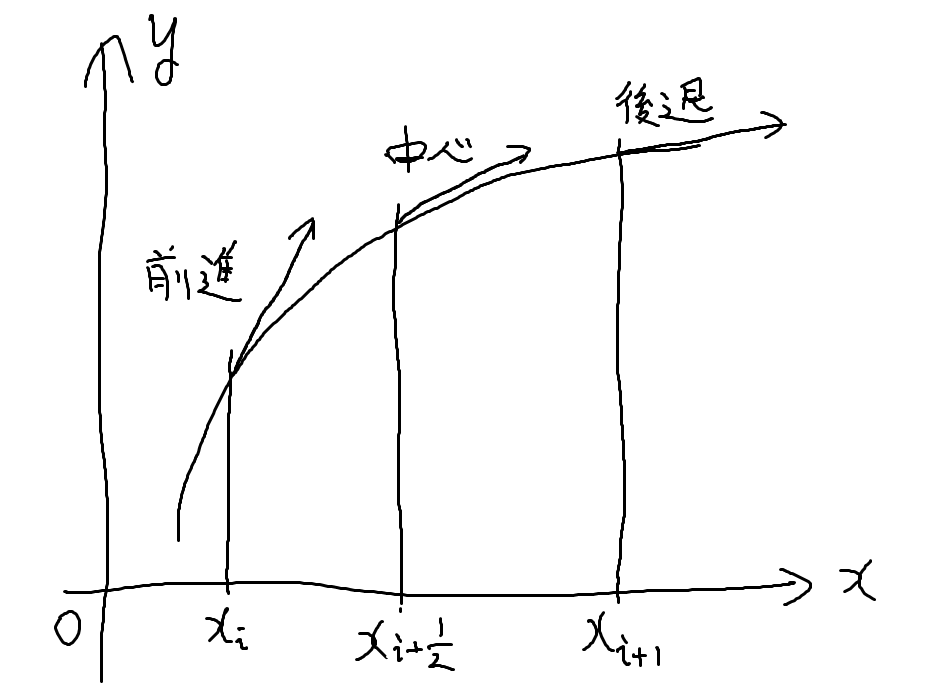
\includegraphics[width=10cm]{img/4-difference.png}
  \caption{差分近似のイメージ}
  \label{fig:4-difference}
\end{figure}

次に二階の導関数を考えましょう。式\ref{eq:advance-taylor}と式\ref{eq:retreat-taylor}を辺々足すと、

\begin{eqnarray}
    y(x+h)+y(x-h)&=&2y(x)+2\frac{h^2}{2!}\frac{\dd^2}{\dd x^2}y(x)+2\frac{h^4}{4!}\frac{\dd^4}{\dd x^4}y(x)+\cdots \\
    \frac{y(x+h)-2y(x)+y(x-h)}{h^2}&=&\frac{\dd^2}{\dd x^2}y(x)+2\frac{h^2}{4!}\frac{\dd^4}{\dd x^4}y(x)
\end{eqnarray}

\noindent
となり、誤差が$O(h^2)$の二階導関数ができました。これは「二階導関数の中心差分近似」と言います。

では微分方程式を解きましょう。微分方程式を$x_i,Y_{i-1}Y_i,Y_{i+1}$を使って書き直すと、これまでの近似から、

\begin{eqnarray}
    \frac{Y_{i+1}-2Y_i+Y_{i-1}}{h^2}=f\pqty{x_i,Y_i,\frac{Y_{i+1}-Y_{i-1}}{2h}}
    \label{eq:difference-original}
\end{eqnarray}

\noindent
となります。このように、差分近似を用いて導いた式を「差分方程式」と言います。また、その解を「差分解」と言います。

少し具体的な方程式として二階線形微分方程式

\begin{eqnarray}
    \frac{\dd^2 y}{\dd x^2}=P(x)\frac{\dd y}{\dd x}+Q(x)y+R(x)
\end{eqnarray}

\noindent
を考えてみましょう。ここで、$P(x)$、$Q(x)$、$R(x)$は既知の関数です。この問題を式\ref{eq:difference-original}を使って書き直すと、

\begin{eqnarray}
    \frac{Y_{i+1}-2Y_i+Y_{i-1}}{h^2}=P(x_i)\frac{Y_{i+1}-Y_{i-1}}{2h}+Q(x_i)Y_i+R(x_i)
\end{eqnarray}

\noindent
となります。これを整理して、

\begin{eqnarray}
    \pqty{1-\frac{1}{2}hP(x_i)}Y_{i+1}-(2+h^2Q(x_i))Y_i+\pqty{1+\frac{1}{2}hP(x_i)}Y_{i-1}=h^2R(x_i)
\end{eqnarray}

\noindent
を得ます。これを、

\begin{eqnarray}
    a_i&=&1+\frac{1}{2}hP(x_i) \\
    b_i&=&-(2+h^2Q(x_i)) \\
    c_i&=&1-\frac{1}{2}hP(x_i)
\end{eqnarray}

\noindent
と置いて、

\begin{eqnarray}
    c_iY_{i+1}+b_iY_i+a_iY_{i-1}=h^2R(x_i)
\end{eqnarray}

\noindent
と書き換えます。この式を$i=1$から$i=N-1$まで並べて書いてみましょう。

\begin{eqnarray}
    \pqty{\begin{array}{ccccc}
        b_1 & c_1 & 0 & 0 & \hdots \\
        a_2 & b_2 & c_2 & 0 & \hdots \\
        0 & a_3 & b_3 & c_3 & \hdots \\
        \vdots & \vdots & \vdots & \vdots & \vdots \\
        \hdots & 0 & a_{N-2} & b_{N-2} & c_{N-2} \\
        \hdots & 0 & 0 & a_{N-1} & b_{N-1}
    \end{array}}
    \pqty{\begin{array}{c}
        Y_1 \\
        Y_2 \\
        Y_3 \\
        \vdots \\
        Y_{N-2} \\
        Y_{N-1}
    \end{array}}
    =\pqty{\begin{array}{c}
        h^2R(x_1)-a_1y_0 \\
        h^2R(x_2) \\
        h^2R(x_3) \\
        \vdots \\
        h^2R(x_{N-2}) \\
        h^2R(x_{N-1})-c_{N-1}y_N
    \end{array}}
    \label{eq:difference-liner-final}
\end{eqnarray}

一番上と一番下の行はそれぞれ定義域の境界なので、境界値を使って

\begin{eqnarray}
    c_1Y_2+b_1Y_1&=&h^2R(x_1)-a_1y_0 \\
    b_{N-1}Y_{N-1}+a_{N-1}Y_{N-2}&=&h^2R(x_{N-1})-c_{N-1}Y_N
\end{eqnarray}

\noindent
の式を用います。

これは単なる連立一次方程式ですね。ここで連立一次方程式の解き方を考えてみましょう。連立一次方程式の数値的な解き方には様々なものがありますが、ここでは式\ref{eq:difference-liner-final}に現れる行列が疎である\footnote{0が多いという意味です}性質を利用して効率的に解く方法(反復法)を2つ紹介します。







\subsubsection{ヤコビ法}
\label{jacobian}
式\ref{eq:difference-liner-final}の行列は常に対角成分$b_i$が0でないとしましょう。すると、$a_i$を含む項と$c_i$を含む項を右辺に移項して、

\begin{eqnarray}
    \pqty{\begin{array}{ccccc}
        b_1 & 0 & 0 & 0 & \hdots \\
        0 & b_2 & 0 & 0 & \hdots \\
        0 & 0 & b_3 & 0 & \hdots \\
        \vdots & \vdots & \vdots & \vdots & \vdots \\
        \hdots & 0 & 0 & b_{N-2} & 0 \\
        \hdots & 0 & 0 & 0 & b_{N-1}
    \end{array}}
    \pqty{\begin{array}{c}
        Y_1 \\
        Y_2 \\
        Y_3 \\
        \vdots \\
        Y_{N-2} \\
        Y_{N-1}
    \end{array}}
    =\pqty{\begin{array}{c}
        h^2R(x_1)-a_1y_0-c_1Y_2 \\
        h^2R(x_2)-a_2Y_1-c_2Y_3 \\
        h^2R(x_3)-a_3Y_2-c_3Y_4 \\
        \vdots \\
        h^2R(x_{N-2})-a_{N-2}Y_{N-3}-c_{N-2}Y_{N-1} \\
        h^2R(x_{N-1})-a_{N-1}Y_{N-2}-c_{N-1}y_N
    \end{array}}
\end{eqnarray}

\noindent
と書き直すことができます。この中から1つ式を取り出すと、

\begin{eqnarray}
    b_nY_n=h^2R(x_n)-a_nY_{n-1}-c_nY_{n+1}
\end{eqnarray}

\noindent
という式になります。これを、

\begin{eqnarray}
    b_iY_i^{(j+1)}=h^2R(x_i)-a_iY_{i-1}^{(j)}-c_iY_{i+1}^{(j)}
\end{eqnarray}

\noindent
と読みかえるとどうでしょう。右辺は$j$回目に計算した$Y$の値、左辺は$j+1$回目に計算した$Y$の値になります。初期値$Y_1^{(0)}$から$Y_{N-1}^{(0)}$を適当に(全部0でOKです)設定してこの式を使って反復的に計算し、十分小さい正の$\epsilon$をによって$|Y_i^{(j)}-Y_i^{(j+1)}|<\epsilon$となったら計算を打ち切りましょう。

このようにして連立一次方程式を数値的に解くことができます。擬似コードを示します。

\begin{algorithm}
\label{al:difference-jacobian}
\caption{差分法(ヤコビ法を使用)}
\begin{algorithmic}
\REQUIRE $x_0,Y_0,Y_N,h,N,\epsilon$
\ENSURE $\boldsymbol{Y}$
\FOR{$i=1$ \TO $N-1$}
    \STATE $\boldsymbol{x}_i\Leftarrow x_{i-1}+h$
    \STATE $\boldsymbol{a}_i\Leftarrow 1+\frac{1}{2}hP(x_i)$
    \STATE $\boldsymbol{b}_i\Leftarrow -(2+h^2Q(x_i))$
    \STATE $\boldsymbol{c}_i\Leftarrow 1-\frac{1}{2}hP(x_i)$
\ENDFOR
\WHILE{at least one $|Y_{i+1}''-Y_{i+1}|\geq\epsilon$}
    \FOR{$i=1$ \TO $N-1$}
        \STATE $Y_i'\Leftarrow Y_i$
        \STATE $Y_i\Leftarrow h^2R(x_i)-\boldsymbol{a}_iY_{i-1}''-\boldsymbol{c}_iY_{i+1}''$
    \ENDFOR
    \FOR{$i=1$ \TO $N-1$}
        \STATE $Y_i''=Y_i'$
    \ENDFOR
\ENDWHILE
\RETURN $\boldsymbol{Y}$
\end{algorithmic}
\end{algorithm}


もう少し一般的に書きましょう。式\ref{eq:difference-liner-final}を、行列$A$、ベクトル$\boldsymbol{Y}$および$\boldsymbol{b}$を用いて書き直すと、

\begin{eqnarray}
    A\boldsymbol{Y}=\boldsymbol{b}
    \label{eq:coalition}
\end{eqnarray}

\noindent
となります。ここで、$A$を一般的に

\begin{eqnarray}
    A=\pqty{\begin{array}{cccc}
        a_{1\ 1} & a_{1\ 2} & \cdots & a_{1\ N} \\
        a_{2\ 1} & a_{2\ 2} & \cdots & a_{2\ N} \\
        \vdots & \vdots & \ddots & \vdots \\
        a_{N\ 1} & a_{N\ 2} & \cdots & a_{N\ N}
        \end{array}}
\end{eqnarray}

\noindent
と置いて、$A=D+M$として$A$を以下の2つの行列に分けましょう。

\begin{eqnarray}
    D=\pqty{\begin{array}{cccc}
        a_{1\ 1} & 0 & \cdots & 0 \\
        0 & a_{2\ 2} & \cdots & 0 \\
        \vdots & \vdots & \ddots & \vdots \\
        0 & 0 & \cdots & a_{N\ N}
        \end{array}},\ 
    M=\pqty{\begin{array}{cccc}
        0 & a_{1\ 2} & \cdots & a_{1\ N} \\
        a_{2\ 1} & 0 & \cdots & a_{2\ N} \\
        \vdots & \vdots & \ddots & \vdots \\
        a_{N\ 1} & a_{N\ 2} & \cdots & 0
        \end{array}}
\end{eqnarray}

すると、

\begin{eqnarray}
    (D+M)\boldsymbol{Y}&=&\boldsymbol{b} \\
    D\boldsymbol{Y}&=&-M\boldsymbol{Y}+\boldsymbol{b} \nonumber \\
    \boldsymbol{Y}&=&-D^{-1}M\boldsymbol{Y}+D^{-1}\boldsymbol{b} \setcounter{equation}{72}
\end{eqnarray}

ここで、左辺を$i+1$回目の計算、右辺を$i$回目の計算とすると、

\begin{eqnarray}
    \boldsymbol{Y}^{(i+1)}&=&-D^{-1}M\boldsymbol{Y}^{(i)}+D^{-1}\boldsymbol{b}
\end{eqnarray}

\noindent
となり、$i$回目の計算で使用した$Y$を再利用して$i+1$回目の計算を行えます。








\subsubsection{ガウス・ザイデル法}
\label{gauss-seidel}
ヤコビ法の収束を早めた方法として、ガウス・ザイデル法があります。ヤコビ法では$Y_i^{(j+1)}$の値を求めるのに$Y_{i+1}^{(j)}$と$Y_{i-1}^{(j)}$の値を使っていましたが、ここで少し考えてみましょう。アルゴリズム\ref{al:difference-jacobian}を見ると、$Y_i^{(j+1)}$を求める時点で$Y_{i-1}^{(j+1)}$が求まっています。$Y_{i-1}^{(j)}$よりも$Y_{i-1}^{(j+1)}$を使った方が収束が早くなります。このように、$j+1$回目の計算をするときになるべく$j+1$回目にすでに行った計算結果を使う手法をガウス・ザイデル法と言います。これを擬似コードにするとヤコビ法より簡潔になります(アルゴリズム\ref{al:difference-gauss-seidel})。

\begin{algorithm}
\label{al:difference-gauss-seidel}
\caption{差分法(ガウス・ザイデル法を使用)}
\begin{algorithmic}
\REQUIRE $x_0,Y_0,Y_N,h,N,\epsilon$
\ENSURE $\boldsymbol{Y}$
\FOR{$i=1$ \TO $N-1$}
    \STATE $\boldsymbol{x}_i\Leftarrow x_{i-1}+h$
    \STATE $\boldsymbol{a}_i\Leftarrow 1+\frac{1}{2}hP(x_i)$
    \STATE $\boldsymbol{b}_i\Leftarrow -(2+h^2Q(x_i))$
    \STATE $\boldsymbol{c}_i\Leftarrow 1-\frac{1}{2}hP(x_i)$
\ENDFOR
\WHILE{at least one $|Y_{i+1}'-Y_{i+1}|\geq\epsilon$}
    \FOR{$i=1$ \TO $N-1$}
        \STATE $Y_i'\Leftarrow Y_i$
        \STATE $Y_i\Leftarrow h^2R(x_i)-\boldsymbol{a}_iY_{i-1}'-\boldsymbol{c}_iY_{i+1}'$
    \ENDFOR
\ENDWHILE
\RETURN $\boldsymbol{Y}$
\end{algorithmic}
\end{algorithm}

ガウス・ザイデル法も行列演算を使って表しましょう。行列$A$を$A=D+L+U$として分解します。ここで$D$はヤコビ法のものと同じで、$L$と$U$はそれぞれ下三角行列と上三角行列で、

\begin{eqnarray}
    L=\pqty{\begin{array}{cccc}
        0 & 0 & \cdots & 0 \\
        a_{2\ 1} & 0 & \cdots & 0 \\
        \vdots & \vdots & \ddots & \vdots \\
        a_{N\ 1} & a_{N\ 2} & \cdots & 0
        \end{array}},\ 
    U=\pqty{\begin{array}{cccc}
        0 & a_{1\ 2} & \cdots & a_{1\ N} \\
        0 & 0 & \cdots & a_{2\ N} \\
        \vdots & \vdots & \ddots & \vdots \\
        0 & 0 & \cdots & 0
        \end{array}}
\end{eqnarray}

\noindent
です。これらを使って元の連立方程式\ref{eq:coalition}を書き直すと、

\begin{eqnarray}
    (D+L+U)\boldsymbol{Y}=\boldsymbol{b} \\
    D\boldsymbol{Y}=-L\boldsymbol{Y}-U\boldsymbol{Y}+\boldsymbol{b} \nonumber \\
    \boldsymbol{Y}=-D^{-1}L\boldsymbol{Y}-D^{-1}U\boldsymbol{Y}+D^{-1}\boldsymbol{b} \setcounter{equation}{76}
\end{eqnarray}

\noindent
となります。ここで、計算回数を明記すると

\begin{eqnarray}
    \boldsymbol{Y}^{(i+1)}=-D^{-1}L\boldsymbol{Y}^{(i+1)}-D^{-1}U\boldsymbol{Y}^{(i)}+D^{-1}\boldsymbol{b}
\end{eqnarray}

\noindent
です。右辺第一項は、下三角行列に$\boldsymbol{Y}$が掛かっているので、$\boldsymbol{Y}$の$i+1$回目の計算が完了している部分です。よって、ここにかかる$\boldsymbol{Y}$は$i+1$回目の計算結果を使用します。






\clearpage